\documentclass[12pt, letterpaper]{article}
\usepackage{graphicx} % Required for inserting images
\usepackage{hyperref}
\usepackage{listings}
\usepackage{amssymb}
\usepackage{amsmath}
\usepackage[english]{babel}
\usepackage{amsfonts}
\usepackage{nicefrac, xfrac}
\usepackage[utf8]{inputenc}
\usepackage{mathtools}
\newcommand{\acc}{\\\hphantom{}\\}
\usepackage[dvipsnames]{xcolor}
\usepackage[titles]{tocloft} % Optional: Better control of the table of contents

\definecolor{light-gray}{gray}{0.95}
\newcommand{\code}[1]{\colorbox{light-gray}{\texttt{#1}}}
\newcommand{\codee}[1]{\colorbox{white}{\texttt{#1}}}
\usepackage[paper=a4paper,left=20mm,right=20mm,bottom=25mm,top=25mm]{geometry}
\renewcommand{\labelenumii}{\arabic{enumi}.\arabic{enumii}}
\renewcommand{\labelenumiii}{\arabic{enumi}.\arabic{enumii}.\arabic{enumiii}}
\renewcommand{\labelenumiv}{\arabic{enumi}.\arabic{enumii}.\arabic{enumiii}.\arabic{enumiv}}
\newcommand{\id}{{\hphantom{ident}}}
\newcommand{\vincolo}[1]{\colorbox{Orange}{$[$\text{#1}$]$}}
\title{\textbf{QuickHospital}}

\date{}

\begin{document}

\maketitle

\tableofcontents 
\newpage
\section{Requisiti}
1. Paziente \\ 
\id 1.1 nome \\
\id 1.2 cognome \\
\id 1.3 data di nascita \\ 
\id 1.4 recapiti telefonici [1..*] \\ 
\id 1.5 email \\ 
\id 1.6 recapito postale  \\
\id 1.7 interno o esterno? \\ 
\id \id 1.7.1 se esterno, prestazione medica richiesta (vedi REQ 4.)
\acc 
2. Medico \\ 
\id 2.1 nome \\ 
\id 2.2 cognome \\ 
\id 2.3 data di nascita \\ 
\id 2.4 pazienti in cura \\ 
\id 2.5 specializzazione primaria\\
\id 2.6 specializzazione secondaria\acc 
3. Ricovero \\ 
\id 3.1 paziente coinvolto \\ 
\id 3.2 stanza del ricovero \\ 
\id \id 3.3 numero posti letto (da 1 a 8)\\
\id \id 3.4 piano \\ 
\id \id 3.5 settore \\ 
\id \id 3.6 data ricovero \acc 
4. Prestazione Medica \\ 
\id 4.1 Paziente esterno coinvolto \\
\id 4.2 data richiesta \\
\id 4.3 specializzazione medica richiesta \\
\id 4.4 descrizione estesa
\newpage 
\section{Diagramma UML delle classi}
\begin{center}
    \includegraphics[width=1\textwidth ]{images/UML.eps}
\end{center}
\section{Tipi di Dato}

\begin{itemize}
    \item $Cell= stringa secondo Regex: '+[0..9]{2} [0..9]{10}$'
    \item $Indirizzo= Tipo di Dato Enum \{via: Stringa, n_civico:int \}$
    \item $Email= stringa secondo Regex: '[A..Za..z]@[a..z].[a..z]'$
\end{itemize}
\newpage 
\section{Vincoli Esterni}
\begin{quote}
    [V.RicoveroTerminato.fineGinizio]
    $$\forall r_t,t_i,t_f \quad RicoveroTerminato(r_t) \wedge DataInizio(r_t,t_i) \wedge DataFine(r_t,t_f)\Rightarrow t_f\ge t_i $$

    [V.Stanza.num\_link]

    Sia $R_s := \{ r | Ricovero(r) \land \lnot RicoveroTerminato(r) \land ric\_st(r,this)\}$\\
    $$|R_s| \le 8$$
    [V.Ricovero.nascita$<$ricovero]
    $$ \forall d_n,d_r,r,p \quad dataNascita(d_n,p)\land DataInizio(d_r,r) \land Paziente(p) \land Ricovero(r)\Rightarrow d_n < d_r$$ 
    
    [V.Prestazione.nascita$<$prestazione]
    $$ \forall d_n,d_p,pr,p \quad dataNascita(d_n,p)\land data(d_r,pr) \land Paziente(p) \land Prestazione(p)\Rightarrow d_n < d_p$$  

    [V.Paziente.ric\_ricterm]
    $$ \not\exists p,r_1,r_2 \quad Paziente(p)\land paz\_ric(p,r_1)\land paz\_ric(p,r_2)\land r_1\neq r_2 \land \lnot RicoveroTerminato(r_1)\land \lnot RicoveroTerminato(r_2)$$
\end{quote}
\section{Operazioni di classe}
\subsection{Operazioni di Stanza}
    \begin{quote}
        postiDisponibili() : Intero $\ge$ 0
        \begin{itemize}
            \item pre: Nessuna
            \item post: Non modifica il livello estensionale dei dati (nessuna nuova ennupla o modifiche a $\mathcal{D}$) \\$M_{in}=M_{out}$.
            \\
            Sia $this,p\quad$ $postiLetto(this,p)$, $Stanza(this)$ e $R:=\{r| ric\_st(r,this) \wedge Ricovero(r)\wedge \lnot RicoveroTerminato(r)\}$.\\
            $$result = p - |R|$$
        \end{itemize}
    \end{quote} \newpage
\section{Specifica degli Use-Case}
\subsection{Diagramma}
\begin{center}
    \includegraphics[width=1\textwidth ]{images/UseCase.eps}
\end{center} \newpage
\subsection{Registra Anagrafica}
    \begin{quote}
        registra\_paziente(n : Stringa, c: Stringa, nascita: Date, tel : $\mathcal{T}$ , email : Email , post: Indirizzo, est : Booleano ): Paziente
        \begin{itemize}
            \item pre: 
            \item post: Modifica il livello estensionale quindi $M_{in} \neq M_{out}$.\\
            Elementi di $\mathcal{D}$ aggiunti : $\rho$\\
            Elementi di $\mathcal{D}$ rimossi : nessuno\\
            Tuple aggiunte:
            \begin{itemize}
                \item $est = true \Rightarrow PazienteEsterno(\rho)$ , altrimenti $Paziente(\rho)\Rightarrow \lnot PazienteEsterno(\rho)$
                \item $nome(\rho, n)$
                \item $cognome(\rho,c)$
                \item $dataNascita(\rho, nascita)$
                \item $recapitoEmail(\rho,email)$
                \item $recapitoPostale(\rho, post)$
                \item $\forall t \in tel \quad recapitoTelefonico(\rho,t)$
            \end{itemize}
            Tuple rimosse : nessuna  \\
            $result = \rho$
        \end{itemize}
    \end{quote}
\subsection{Registra richiesta di prestazione}
    \textbf{registra\_prestazione($\rho$: PazienteEsterno, $d$ : Stringa, $s$: Specializzazione, $\delta$ : Data) : Prestazione}
    \begin{itemize}
        \item pre : Sia $D :=\{ [d_i,d_f] \quad| Data(d_f)\land Data(d_i) \land paz\_ric(p,r)\land RicoveroTerminato(r) \land DataFine(r,d_f) \land DataInizio(r,d_i)\}$\\
        $\delta \notin [d_i^j,d_f^j] \quad \forall d_i^j, d_f^j \in D$
        \item post : $M_{in} \neq M_{out}$\\
        Elementi di $\mathcal{D}$ aggiunti: $p$\\
        Elementi di $\mathcal{D}$ rimossi: nessuno \\
        Tuple aggiunte:
        \begin{itemize}
            \item $descrizione(d,p)$
            \item $data(\delta,p)$
            \item $paz\_prest(\rho,p)$
            \item $prest\_spec(p,s)$
        \end{itemize}
        $result = p$
    \end{itemize}

 \textbf{lista\_medici($\pi$: Prestazione): Medico[0..*]}
    \begin{itemize}
        \item pre: nessuna
        \item post : $M_{in} = M_{out}$\\
        Sia $\mathcal{M} :=\{ m\quad | \exists s \quad Medico(m)\land Specializzazione(s)\land prest\_spec(\pi,s)\land primaria(s,m)\}$.\\
        Sia $\mathcal{M}_s := \{ m\quad | \exists s \quad Medico(m)\land Specializzazione(s)\land prest\_spec(\pi,s)\land secondaria(s,m)\}$.\\
        $|\mathcal{M}|> 0 \Rightarrow result = \mathcal{M}$ \\
        $\land$\\
        $|\mathcal{M}|=0 \rightarrow result = \mathcal{M}_s$
    \end{itemize}

\subsection{Registra ricovero}
    \textbf{registra\_ricorvero($\rho$: Paziente, $\mu$ : Medico, $d$ : Data): Ricovero}
    \begin{itemize}
        \item pre: Sia $S : =\{(s,p) | Stanza(s)\land postiDisponibili(s,p)\land p>0 \}$, $\displaystyle\sigma = \sum_{(s,p)\in S} p$\\
        $$\sigma > 0$$
        \item post: $M_{in} \neq M_{out}$\\
        Elementi di $\mathcal{D}$ aggiunti: $\omega$\\
        Elementi di $\mathcal{D}$ rimossi: nessuno \\
        Tuple aggiunte:
        \begin{itemize}
            \item DataInizio($\omega$,$adesso$)
            \item $med\_ric(\mu,\omega)$
            \item $paz\_ric(\rho, \omega)$
            \item Sia $S:=\{s | Stanza(s) \land postiDisponibili(s)>0\}$, scelta arbitraria di $s\in S$, $ric\_st(\omega, s)$.
        \end{itemize}
        $result = \omega$
    \end{itemize}

    \textbf{registra\_dimissione($r$: Ricovero, $\delta$: Data): RicoveroTerminato}
    \begin{itemize}
        \item pre:  Sia $d_i$, $DataInizio(r,d_i)\Rightarrow \delta>d_i$ $\land \lnot RicoveroTerminato(r)$
        \item post: $M_{in}\neq M_{out}$\\
        Elementi di $\mathcal{D}$ aggiunti: nessuno\\
        Elementi di $\mathcal{D}$ rimossi: nessuno \\
        Tuple aggiunte:
        \begin{itemize}
            \item $RicoveroTerminato(r)$
            \item $datFine(r,\delta)$
        \end{itemize}
        $result = r$
    \end{itemize}
\subsection{Calcola itinerario}
\begin{quote}
    itinerario(m : Medico): $\mathcal{I}$
    \begin{itemize}
        \item pre : Sia $m$ l'istanza di Medico che rappresenta l'attore che invoca l'operazione
        \item post: $M_{in} = M_{out}$\\
        Sia $R := \{ r | Ricovero(r) \land \lnot RicoveroTerminato(r)\land  med\_ric(m,r)\}$\\
        Sia $S := \{ s | \exists r\in R \land Stanza(s) \land ric\_st(r,s)\}$\\
        Sia $T := \{(p,\sigma) | \exists s\in S \land piano(s,p) \land settore(s,\sigma)\}$\\
        $result = \mathcal{I}_T$
    \end{itemize}
\end{quote}
\newpage

Arrivati a questo punto la fase di \textbf{Analisi} è \textbf{finita}.
\section{Ristrutturazione}
\subsection{Diagramma UML ristrutturato}
\begin{center}
    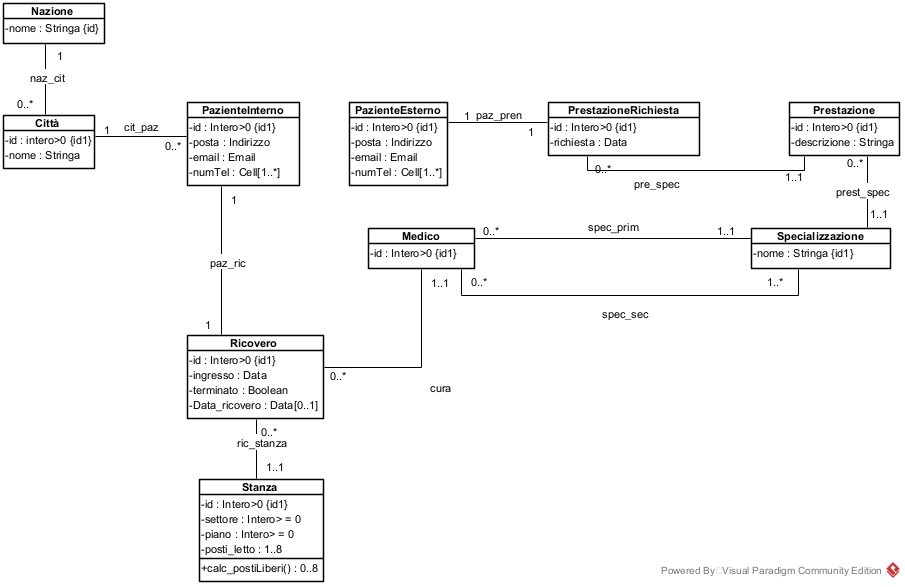
\includegraphics[width=1\textwidth ]{images/Ristrutturato.jpg}
\end{center}
\textbf{Modifiche sulle generalizzazioni effettuate:}
\begin{itemize}
    \item Generalizzazione PazienteEsterno$-$PazienteInterno: \\
    E' stata preferita la divisione tra pazienti interni ed esterni poichè è più facile e veloce nella ricerca avere due tabelle separate.\\
    Se un paziente è sia interno che esterno, avrò 2 tuple uguali sulle due tabelle.
    \item Generalizzazione Ricovero$-$RicoveroTerminato: \\
    La generalizzazione per RicoveroTerminao è stata eliminata.
    \item Generalizzazione SpecializzazionePrimaria$-$SpecializzazioneSecondaria: \\
    La generalizzazione tra SpecializzazionePrimaria e SpecializzazioneSecondaria è stata eliminata e aggiunto un vincolo esterno.\\

\end{itemize}

\newpage
\subsection{Tipi e Domini}
\subsubsection{Tipi}
\begin{itemize}
    
    \item create type Indirizzo as enum \{
        via: varchar(100),
        n$\_$civico: Intero$>$0,
    \}

\end{itemize}
\subsubsection{Domini}
\begin{itemize}
    \item create domain Intero$>$0 as integer check(value$>$0 not NULL)
    \item create domain Telefono as integer secondo regex ('$+[1..9]\{2\}$ $[0..9]\{10\}$')
    \item create domain Email as varchar secondo regex ('[a..zA..Z]@[a..z].[a..z]') 
\end{itemize}
\subsection{Vincoli Esterni}
I precedenti vincoli esterni non violano la nuova ristrutturazione.\\
Nuovi vincoli esterni:\\
\begin{quote}
    [V.Medico.specializzazioni]\\
        Data Una SpecializzazionePrimaria essa non può essere SpecializzazioneSecondaria per lo stesso medico.\\
        $$\forall m, s Medico(m) \land Specializzazione(s) \land SpecializzazionePrimaria(m,s)$$\\ $$\rightarrow \lnot SpecializzazioneSecondaria(m,s)$$
\end{quote}
\subsection{Use Case}
Gli use case non violano la nuova ristrutturazione.
\newpage
\subsection{Traduzione diretta del diagramma UML delle classi ristrutturato}
Saranno scritte tutte le tabelle da creare.
\begin{itemize}
    \item Nazione(\underline{\textbf{nome}}: Stringa)
    \item Citta(\underline{\textbf{id}}: nome, nazione: Nazione)
    \begin{itemize}
        \item fk: nazione references Nazione(\underline{\textbf{nome}})
    \end{itemize}
    \item PazienteInterno(\underline{\textbf{id}}: intero>0, posta: Indirizzo, email: Email, numTel, citta\_residenza: Citta)
    \begin{itemize}
        \item fk: citta\_residenza references Citta(\underline{\textbf{id}})
    \end{itemize}
    \item Ricovero(\underline{\textbf{id}}: integer, ingresso: Date, terminato: Boolean: data\_ricovero*, stanza: Stanza, specialista: Medico)
    \begin{itemize}
        \item // UNISCO A STANZA PER AVERE UNA TABELLA CON LE INFORMAZIONI UNICHE DI UN RICOVERO
        \item // UNISCO A MEDICO PER AVERE OGNI RICOVERO LE INFORMAZIONI DEL MEDICO
        \item fk: stanza references Stanza(\underline{\textbf{id}})
        \item fk: specialista references Medico(\underline{\textbf{id}})
    \end{itemize}
    \item paz\_ric(paz: Paziente, ric: Ricovero)
    \begin{itemize}
        \item //LO TENGO PERCHè VOGLIO UNA TABELLA CON LA LISTA DEI PAZIENTI ATTUALMENTE RICOVERATI
        \item foreign key: paz references Paziente(\underline{\textbf{id}})
        \item foreign key: ric references Ricovero(\underline{\textbf{id}})
    \end{itemize}
    \item Stanza(\underline{\textbf{id}}: integer, settore: intero>0, piano: intero>=0 posti\_letto: 1..8)
    \item PazienteEsterno(\underline{\textbf{id}}: integer, posta: Indirizzo, email: Email, numTel, prenotazione: PrenotazioneRichiesta)
    \begin{itemize}
        \item fk: prenotazione references PrenotazioneRichiesta(\underline{\textbf{id}})
        \item // UNISCO PER AVERE UNA TABELLA CON I PAZIENTI ESTERNI DIRETTAMENTE COLLEGATA ALLA PRENOTAZIONE
    \end{itemize}
    \item PrenotazioneRichiesta(\underline{\textbf{id}}, richiesta: Date, prestazione: Prestazione)
    \begin{itemize}
        \item fk: prestazione references Prestazione(\underline{\textbf{id}})
        \item // UNISCO PER AVERE UNA TABELLA CON LE PRENOTAZIONI DIRETTAMENTE COLLEGATA ALLE PRESTAZIONI
    \end{itemize}
    \item Prestazione(\underline{\textbf{id}}: integer, descrizione: varchar(100), spec: Specializzazione)
    \begin{itemize}
        \item fk: spec references Specializzazione(\underline{\textbf{nome}})
    \end{itemize}
    \item Specializzazione(\underline{\textbf{nome}}: varchar(100))
    \item Medico(\underline{\textbf{id}}: integer, spec\_prim: Specializzazione)
    \begin{itemize}
        \item fk: spec\_prim references Specializzazione(\underline{\textbf{nome}})
        \item v.inclusione Medico(\underline{\textbf{id}}) occorre in spec\_sec(Medico)
    \end{itemize}
    \item spec\_sec(Medico: intero, Specializzazione: varchar(100))
    \begin{itemize}
        \item foreign key: Medico references Medico(\underline{\textbf{id}})
        \item foreign key: Specializzazione references Specializzazione(\underline{\textbf{nome}})
    \end{itemize}
    \item // UNISCO MEDICO E SPECIALIZZAZIONE PRIMARIA, LASCIO UNA TABELLA SEPARATA PER LE SPECIALIZZAZIONI SECONDARIE
\end{itemize}
\newpage
\subsection{Trigger}
I vincoli esterni da controllare con i trigger sono:

\subsubsection{V.Medico.specializzazioni}
\begin{verbatim}
Trigger per il vincolo V.Medico.specializzazioni:
    Operazioni: inserimento o modifica in Medico o in spec_sec
    Istante di invocazione: prima dell'operazione intercettata
    Funzione:
        Sia isError=FALSE;
        Sia new l’ennupla che si sta inserendo oppure l’ennupla risultato della modifica;
        Se si sta inserendo o modificando una ennupla in Medico:
            isError:= exists(select * 
                            from Medico m, spec_sec s 
                            where m.id=new.id 
                            and m.spec_prim=s.Specializzazione and s.Medico=new.id)
        
        Se si sta inserendo o modificando una ennupla in spec_sec:
            isError:= exists(select * 
                            from Medico m, spec_sec s 
                            where m.id=new.Medico 
                            and m.spec_prim=s.Specializzazione and s.Medico=new.Medico)
        
        Se isError = TRUE blocca l’operazione;
        Altrimenti permetti l’operazione
\end{verbatim}
\subsubsection{V.Ricovero.fineGinizio}
\begin{verbatim}
Trigger per il vincolo V.Ricovero.fineGinizio:
    Operazioni: inserimento o modifica in Ricovero
    Istante di invocazione: prima dell'operazione intercettata
    Funzione:
        Sia isError=FALSE;
        Sia new l’ennupla che si sta inserendo oppure l’ennupla risultato della modifica;
        isError:= exists(select * 
                        from Ricovero r
                        where r.id=new.id 
                        and r.igresso>new.data_ricovero)
        
        Se isError = TRUE blocca l’operazione;
        Altrimenti permetti l’operazione
\end{verbatim} \newpage
\subsubsection{V.Stanza.num\_link}
\begin{verbatim}
Trigger per il vincolo V.Stanza.num_link:
    Operazioni: inserimento o modifica in Stanza
    Istante di invocazione: prima dell'operazione intercettata
    Funzione:
        Sia isError=FALSE;
        Sia new l’ennupla che si sta inserendo oppure l’ennupla risultato della modifica;
        isError:= exists(select count(r)
                        from Stanza s, Ricovero r
                        where s.id=new.id and r.stanza= s.id and r.terminato=false)
        Se isError = TRUE blocca l’operazione;
        Altrimenti permetti l’operazione
\end{verbatim}
\subsubsection{V.Ricovero.nascita$<$ricovero}
\begin{verbatim}
Trigger per il vincolo V.Ricovero.nascita$<$ricovero:
    Operazioni: inserimento o modifica in Ricovero e PazienteInterno
    Istante di invocazione: prima dell'operazione intercettata
    Funzione:
        Sia isError=FALSE;
        Sia new l’ennupla che si sta inserendo oppure l’ennupla risultato della modifica;
        isError:= exists(select * 
                        from Ricovero r, Paziente p
                        where r.id=new.id and r.paziente=p.id and p.nascita<new.data_ricovero)
        Se isError = TRUE blocca l’operazione;
        Altrimenti permetti l’operazione
\end{verbatim}
\subsubsection{V.PazienteEsterno.nascita$<$PrenotazioneRichiesta.richiesta}
\begin{verbatim}
Trigger per il vincolo V.PazienteEsterno.nascita$<$PrenotazioneRichiesta.richiesta:
    Operazioni: inserimento o modifica in PazienteEsterno e PrenotazioneRichiesta
    Istante di invocazione: prima dell'operazione intercettata
    Funzione:
        Sia isError=FALSE;
        Sia new l’ennupla che si sta inserendo oppure l’ennupla risultato della modifica;
        isError:= exists(select * 
                        from PazienteEsterno p, PrenotazioneRichiesta pr
                        where p.id=new.id and p.prenotazione=pr.id and p.nascita<pr.richiesta)
        Se isError = TRUE blocca l’operazione;
        Altrimenti permetti l’operazione
\end{verbatim}\newpage
\subsubsection{V.Paziente.ric\_ricterm}
\begin{verbatim}
Trigger per il vincolo V.Paziente.ric_ricterm:
    Operazioni: inserimento o modifica in Paziente e Ricovero
    Istante di invocazione: prima dell'operazione intercettata
    Funzione:
        Sia isError=FALSE;
        Sia new l’ennupla che si sta inserendo oppure l’ennupla risultato della modifica;
        isError:= exists(select * 
                        from Paziente p, Ricovero r1, Ricovero r2
                        where p.id=new.id and r1.paziente=p.id and r2.paziente=p.id 
                        and r1.id!=r2.id and r1.terminato=false and r2.terminato=false)
        Se isError = TRUE blocca l’operazione;
        Altrimenti permetti l’operazione
\end{verbatim}
\end{document}